\documentclass[11pt,a4paper]{article}

\usepackage{epsfig}
\usepackage{multicol}

\usepackage[utf8]{inputenc}
\usepackage[brazil]{babel}
\usepackage{fancyheadings}
\usepackage{amsmath}
\usepackage{amssymb}
\usepackage{enumerate}
\DeclareGraphicsExtensions{.png,.pdf}
\usepackage{graphicx}
\usepackage{multicol}
\usepackage{graphicx}

% As margens
\setlength{\textheight}{24.0cm}
\setlength{\textwidth}{17.5cm}
\setlength{\oddsidemargin}{2.0cm} % Margens reais desejadas
\setlength{\evensidemargin}{2.0cm} % 2+17.5+1.5=21cm (largura A4)
\setlength{\topmargin}{1.5cm} % 1.5+1.6+1.0+24.0+1.6=29.7cm
\setlength{\headheight}{1.6cm} % (altura A4)
\setlength{\headsep}{1.0cm}
\setlength{\columnsep}{1.5cm} % Coluna = 8cm ((17.5-1.5)/2)
\addtolength{\oddsidemargin}{-1in}
\addtolength{\evensidemargin}{-1in}
\addtolength{\topmargin}{-1in}
\setlength{\footskip}{0.0cm}
\usepackage{tasks}

\newcommand{\mat}[1]{\mbox{\boldmath{$#1$}}} 

\pagestyle{fancy}

\usepackage{lipsum}

\lhead{

\includegraphics[width=1cm]{brasao.png}
}

\rhead{ 
\sc\textbf{U}niversidade \textbf{F}ederal do \textbf{C}eará\\
Campus Quixadá\\ Monitoria de Cálculo II e Cálculo III}

\begin{document}
	
	\begin{center}
		\Large Lista 1 - Cálculo III
	\end{center}		
	
	\begin{enumerate}

		\item No cálculo vetorial temos basicamente 4 tipos de operações diferenciais usando o operador
			$\nabla$, definido como:
			
			$$\nabla = \left(\dfrac{\partial }{\partial x} \textrm{\ ,} \dfrac{\partial }{\partial y} \textrm{\ ,}  \dfrac{\partial }{\partial z} \right)$$ 
			O operador $\nabla$ aplicado a campos de natureza diferentes produz outros campos resultantes como o Gradiente, Divergente, Rotacional e Laplaciano. Utilize a matriz de mudança de base de coordenadas abaixo

$$\hat{\textbf{i}} = \cos \theta \hat{\mat{\rho}} - \sin \theta \hat{\mat{\theta}}$$
$$\hat{\textbf{j}} = \sin \theta \hat{\mat{\rho}} + \cos \theta \hat{\mat{\theta}}$$			
			
			 e seus conhecimentos adquiridos em Cálculo 2 e DEMONSTRE todos os operadores em coordenadas polares, cilíndricas e esféricas. Basicamente verifique que para coordenadas polares:
			 
			 $$\nabla = \hat{\mat{\rho}} \dfrac{\partial }{\partial \rho} + \displaystyle\dfrac{\hat{\mat{\theta}}}{\rho} \dfrac{\partial }{\partial \theta} $$
			
			Depois disso aplique cada operador diferencial a cada campo correspondente e conclua. Cada coordenada terá seu $\nabla$ escrito de forma diferente. O exemplo acima foi apenas para coordenadas polares. Abaixo está o que você deve chegar aproximadamente
			
\begin{figure}[h]

\centering % para centralizarmos a figura
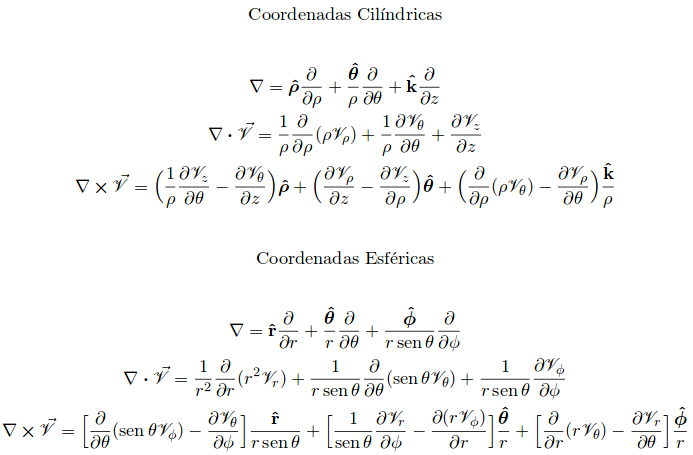
\includegraphics[width=12cm]{Selection_002.png} % leia abaixo
\end{figure}	
	
		\item Calcule o rotacional dos campos vetoriais abaixo:
			\begin{enumerate}
			\item $\overrightarrow{F}(x,y,z) = -y\vec{i} + x\vec{j} + z\vec{k}$
			\item $\overrightarrow{F}(x,y,z) = x\vec{i} + y\vec{j} + xz\vec{k}$
			\item $\overrightarrow{F}(x,y,z) = yz\vec{i} + xz\vec{j} + xy\vec{k}$
			\item $\overrightarrow{F}(x,y) = (x^2 + y^2)\vec{i}$
			\item $\overrightarrow{F}(x,y) = xy\vec{i} - x^2\vec{j}$
			\end{enumerate}
			
			\item Seja $\varphi : \Omega \subset \mathbb{R}^2 \to \mathbb{R}$, $\Omega$ aberto, de classe $C^2$. Verifique que o campo vetorial $\overrightarrow{F} = \nabla \varphi $ é irrotacional.
			
			\item O potencial elétrico numa chapa circular de raio R vale em determinado instante:
	$$V(\rho,\theta) = \displaystyle\dfrac{200 \sin \theta}{\rho + 1}$$
	Determine a taxa de variação do potencial elétrico na direção radial em $P\left(2,\displaystyle\dfrac{\pi}{4}\right)$.
	
	\item Num tanque, na região próxima ao ralo, há um fluido escoando, de modo que seu campo de velocidades vale em coordenadas cilíndricas
	$$\vec{v} = \displaystyle\dfrac{2}{1+\rho} \hat{\mat{\theta}} - 2(4 - z)\hat{\textbf{k}}$$
	onde $\rho$ é a distância de um ponto do fluido ao eixo do ralo, que corresponde ao eixo $z$. A origem está exatamente no centro do ralo, que é uma circunferência de raio $R$.
	A vorticidade de um fluido é dada por $\xi = \nabla \times \vec{v}$. Ache a vorticidade do fluido acima. Se lembre de usar as coordenadas apropriadas ao problema. O escoamento do fluido é irrotacional? Justifique.
	
	\item Mostre que para um corpo rígido girando em torno de um eixo fixo com velocidade angular $\vec{\omega}$, onde as partículas têm velocidades dadas por $\vec{v} = \vec{\omega} \times \vec{r}$, tem-se
	$$\nabla \times \vec{v} = 2\vec{\omega}$$
	Lembre que $\vec{\omega}$ é função apenas de t.
	
	\item Considere o escoamento bidimensional
	$$\overrightarrow{V}(x,y) = \displaystyle\dfrac{-y}{x^2 + y^2} \vec{i} + \displaystyle\dfrac{x}{x^2 + y^2}\vec{j}$$.
	\begin{enumerate}
	\item Desenhe tal campo.
	\item Calcule $\nabla \times \vec{v}$ e interprete.
	\end{enumerate}
	
	\item Calcule o divergente do campo vetorial dado.
	\begin{enumerate}
	\item $\vec{v}(x,y) = -y\vec{i} + x\vec{j}$
	\item $\vec{u}(x,y,z) = x\vec{i} + y\vec{j} + z\vec{k}$
	\item $\overrightarrow{F}(x,y,z) = (x^2 - y^2)\vec{i} + \sin (x^2 + y^2)\vec{j} + \arctan z \vec{k}$
	\item $\overrightarrow{F}(x,y,z) = (x^2 + y^2 + z^2)\arctan (x^2 + y^2 + z^2) \vec{k}$
	
	\end{enumerate}
	
	\item Mostre que:
	
	\begin{enumerate}
	\item $\nabla \ . \ (\nabla \times A) = 0 $
	\item $\nabla \times (\nabla \varphi) = 0 $
	\item $\nabla \times (A + B) = (\nabla \times A) + (\nabla \times B)$
	\item $\nabla \ . \ (A + B) = (\nabla \ . \ A) + (\nabla \ . \ B)$
	\item $\nabla \times (\nabla \times A) = \nabla \ . \ (\nabla \ . \ A) - \nabla ^2 A $
	\end{enumerate}
	
	\item O campo elétrico gerado por uma carga puntiforme é dado pela seguinte relação:
	
	$$\vec{E} = \displaystyle\dfrac{1}{4 \pi \varepsilon_0} \displaystyle\dfrac{Q}{\vec{(d)}^2} \vec{|r|}$$
	
	onde $\varepsilon_0$ é uma constante, $Q$ é a carga da partícula (também constante) e $d$ é a distância da carga geradora até um ponto considerado. $r$ é um versor no ponto. Considere $\vec{d} = {r - r'}$. Costumamos dizer que  quando o rotacional de um campo é igual a zero, então afirmamos que esse campo vetorial é considerado conservativo, ou seja:
	$$\nabla \times \vec{E} = 0$$
	Prove que o campo elétrico gerado por uma carga puntiforme é conservativo. Justifique seus resultados. Lembre-se que com a devida substituição, o rotacional se aplica na variável $r$.
			
	\end{enumerate}
\end{document}